\documentclass[11pt,a4paper]{article}
\usepackage[T1]{fontenc}
\usepackage[utf8]{inputenc}
\usepackage{lmodern}
\usepackage[margin=20mm,top=22mm,bottom=22mm,headheight=15pt]{geometry}
\usepackage{amsmath,amssymb,booktabs,array,graphicx,microtype,tabularx}
\usepackage[dvipsnames]{xcolor}
\usepackage{enumitem,fancyhdr,tcolorbox}
\usepackage[colorlinks=true,linkcolor=MidnightBlue,urlcolor=MidnightBlue,citecolor=MidnightBlue]{hyperref}
\definecolor{courseblue}{HTML}{164B69}
\definecolor{pale}{HTML}{F0F5F7}
\pagestyle{fancy}
\fancyhf{}
\fancyhead[L]{\small\sffamily\color{courseblue}VALIDATED COMPUTING}
\fancyhead[R]{\small\sffamily Applications for Lectures 07--14}
\fancyfoot[L]{\footnotesize Proposals and worked notebooks \textbullet\ November 2026}
\fancyfoot[R]{\footnotesize\thepage}
\renewcommand{\headrulewidth}{0.4pt}
\setlength{\parindent}{0pt}
\setlength{\parskip}{5pt plus 1pt}
\setlength{\emergencystretch}{2em}
\setlist[itemize]{leftmargin=1.5em,itemsep=2pt,topsep=3pt}
\setlist[enumerate]{leftmargin=1.7em,itemsep=3pt,topsep=3pt}
\newcommand{\R}{\mathbb R}
\newcommand{\nb}[1]{\texttt{\detokenize{#1}}}
\newtcolorbox{teaching}[1][Teaching notes]{colback=pale,colframe=courseblue!55,boxrule=0.4pt,
 arc=1mm,left=7pt,right=7pt,top=4pt,bottom=4pt,title={#1},fonttitle=\bfseries\small,
 coltitle=courseblue,colbacktitle=pale}
\newcommand{\lecture}[2]{\section*{\color{courseblue}Lecture #1 \quad #2}\addcontentsline{toc}{section}{Lecture #1: #2}}
\newcommand{\app}[2]{\subsection*{#1\hfill{\small\sffamily\color{black!60}#2}}\addcontentsline{toc}{subsection}{#1}}
\newcommand{\field}[1]{\textbf{\sffamily\small\color{courseblue}#1.}\ }
\hypersetup{pdftitle={Applications for Lectures 07-14},pdfauthor={Validated Computing course}}

\begin{document}

{\LARGE\sffamily\bfseries\color{courseblue}Applications for Lectures 07--14\par}
\vspace{4pt}
{\large Proposals, worked notebooks, and teaching notes\par}
\vspace{6pt}

The lectures from 07 onwards introduce powerful tools (mean-value forms, automatic differentiation,
interval Newton, Krawczyk, branch and bound, filtered predicates) but illustrate them mostly on
textbook functions such as $x(1-x)$, $x^2-2$, a cubic, or the circle meeting the line $y=x$. This document
proposes applications in which the same tools answer questions that matter outside the course, and in
which a floating-point computation gives a visibly wrong or unsupported answer.

Seven proposals are implemented as notebooks in the \nb{applications/} folder (one per lecture,
07--13). The others are described in enough detail to be assigned as projects. Every implemented
notebook runs on the existing \nb{vc} package without changes, follows the course conventions
(Jupytext pair, Colab setup cell, theory and experiment alternating, an explicit failure case), and
ends with four exercises. Background for all of it is in Tucker's book \cite{tucker}.

\begin{center}
\small
\begin{tabularx}{\linewidth}{@{}l X l l@{}}
\toprule
Lecture & Application & Notebook & Run time\\
\midrule
07 & Certified error of a math-library polynomial for $\sin$ & \nb{app07_approximation_error} & 10 s\\
08 & Robustness certificate for a small neural network & \nb{app08_network_robustness} & 5 s\\
09 & First hit of a ray with a torus; all roots of Wilkinson's polynomial & \nb{app09_ray_tracing_and_wilkinson} & 20 s\\
10 & Robot arm reaching a whole path; Hénon periodic orbits & \nb{app10_robot_arm_and_henon} & 15 s\\
11 & Global frequency fit; aliasing found by the certificate & \nb{app11_curve_fitting} & 10 s\\
12 & A convex hull that leaves an input point outside & \nb{app12_convex_hull} & 5 s\\
13 & Audit of four seeded certificates & \nb{app13_seeded_audit} & 2 s\\
\bottomrule
\end{tabularx}
\end{center}
{\footnotesize Run times are approximate, for an unloaded laptop with the course environment.\par}

\paragraph{How to use them.} Each notebook supports three uses. (1) \emph{In-lecture demonstration}:
run it top to bottom in 15--20 minutes after the corresponding theory. (2) \emph{Lab extension}:
assign it as an extra task after the existing Lab tasks A--C. (3) \emph{Homework or mini-project}:
the four exercises at the end grow from routine (rerun with a parameter change) to open-ended (extend
the method). The notebooks are complete worked examples, not starters with stubs; if graded starters
are wanted, the natural cells to blank out are named in each teaching-notes box.

\tableofcontents

%=====================================================================
\newpage
\lecture{07}{Better enclosures}

\app{How accurate is a math-library polynomial?}{implemented: \nb{app07_approximation_error}}

\field{Problem} After argument reduction a math library evaluates a short polynomial $p$ instead
of $\sin x$. The library is correct only if the approximation error $\sup_{x\in D}|\sin x-p(x)|$ is below
the target accuracy on the \emph{whole} reduced range $D$; tools such as Sollya certify exactly this \cite{chevillard}. We take the degree-7 Taylor polynomial and
$D=[0,4/5]\supseteq[0,\pi/4]$.

\field{Why floating point is not enough} Sampling $10^4$ points finds the maximum
$3.677\cdot10^{-7}$ at the right endpoint, but says nothing about the points between samples. A sample
evaluated rigorously gives only a \emph{lower} bound for the supremum.

\field{Certificate} On a piece $X$ of width $h$, natural evaluation of $e=\sin-p$ subtracts two
enclosures of width $\approx h$ and gets width $\approx 2h$: the cancellation that Lecture 06 calls the
dependency problem. The mean-value form $e(X)\subseteq e(m)+e'(X)(X-m)$ moves the large parts into
the sharp point value $e(m)$. Since $e'=\cos-p'$ cancels in the same way, the notebook applies the
mean-value form a second time to $e'$, which is a second-order Taylor bound with a rigorous remainder.

\field{Results} Uniform subdivision of $D$, Arb at 80 bits:

\begin{center}
\small
\begin{tabular}{rccc}
\toprule
pieces & natural & mean value & nested mean value\\
\midrule
16 & $5.0\cdot10^{-2}$ & $9.4\cdot10^{-4}$ & $3.1\cdot10^{-5}$\\
256 & $3.1\cdot10^{-3}$ & $4.1\cdot10^{-6}$ & $3.747\cdot10^{-7}$\\
1024 & $7.8\cdot10^{-4}$ & $6.0\cdot10^{-7}$ & $3.678\cdot10^{-7}$\\
\bottomrule
\end{tabular}
\end{center}

With 1024 pieces, $\sup|e|\in[3.6772492,\,3.6783577]\cdot10^{-7}$, a relative gap of $0.03\%$. That is
about six binary32 ulps near $\sin(4/5)$, so the polynomial is not even good enough for single
precision on the whole range. Natural evaluation would need about $10^7$ pieces for the same result.
A final experiment shows that at 20 bits of working precision the bound stalls at $5.8\cdot10^{-6}$:
the derivative tricks remove dependency, not rounding.

\begin{center}
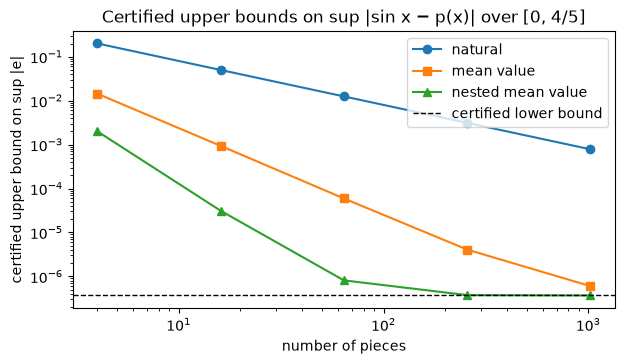
\includegraphics[width=0.78\linewidth]{figures/app07-bounds.png}
\end{center}

\begin{teaching}
The key discussion point is \emph{why} the mean-value form helps here when Lecture 07 also showed it
can be worse: the large terms of $e$ cancel exactly, and the form evaluates them only at a point.
Ask students to predict the slopes of the three lines in the log--log plot ($h$, $h^2$, $h^3$ until
the true supremum is reached). For a graded starter, blank out \nb{second_order} and the table loop.
Exercise 2 (change the $x^7$ coefficient) leads to minimax approximation and the Remez algorithm, a
good bridge to numerical analysis courses.
\end{teaching}

\app{Safe operating envelope}{proposal}

Prove that a quantity stays below a threshold for a whole range of parameters, for example that a
projectile's range $R(\theta)=v^2\sin(2\theta)/g$ with drag correction, or a beam deflection, never
exceeds a limit for every angle or load in an interval. Use \nb{adaptive_range} with a mean-value
evaluator; inconclusive pieces become ``this sub-range needs a better model or a smaller tolerance''.
Effort: one lab session; no new \nb{vc} code. The teaching value is the shape of the output: a
partition of the parameter range into \emph{certified safe}, \emph{certified unsafe} and
\emph{undecided}.

%=====================================================================
\lecture{08}{Automatic differentiation}

\app{Certify that a small neural network is robust}{implemented: \nb{app08_network_robustness}}

\field{Problem} A classifier is robust at $x$ with radius $\varepsilon$ if its decision is constant on
the box $\|x'-x\|_\infty\le\varepsilon$. Attacks \cite{goodfellow} can only refute robustness; a proof needs an enclosure of
the score over the whole box, the starting point of interval bound propagation \cite{gowal}. The notebook uses a $2\to3\to1$ network with $\tanh$ units and exact
rational weights. Since \nb{Dual} supports \nb{exp}, the notebook writes
$\tanh z=1-2/(e^{2z}+1)$, so one Python function serves floats, Arb balls and dual numbers.

\field{Certificate} Three enclosures of the score on a box: natural Arb evaluation; the
two-variable mean-value form with a gradient enclosure from two dual-number passes; and a
\emph{monotone-corner} test: if both partial derivatives have a fixed sign on the box, the minimum and
maximum are attained at two known corners, so two point evaluations suffice. The largest certified
radius is found by bisection on $\varepsilon$, each candidate radius being checked by an actual
certificate. A gradient-sign attack (FGSM) gives an upper bound, and its counterexample corner is
itself verified with Arb.

\field{Results} Largest certified radius by method, and the interval for the true robust radius:

\begin{center}
\small
\begin{tabular}{lcccc}
\toprule
point & natural & mean value & monotone corners & robust radius in\\
\midrule
far (score $+4.46$) & 0.3046 & 0.1215 & 0.3046 & $[0.3046,\,0.3946]$\\
near (score $+0.76$) & 0.0483 & 0.0350 & 0.0562 & $[0.0562,\,0.0562]$\\
very near (score $+0.12$) & 0.0085 & 0.0086 & 0.0097 & $[0.0097,\,0.0097]$\\
\bottomrule
\end{tabular}
\end{center}

Near the decision boundary the certificate meets the attack to four digits: the robust radius is
known. On a large box the mean-value form is \emph{worse} than natural evaluation, because $\tanh$
saturates and the gradient bound over a big box is loose. This is Lecture 07's ``the centered form can
be worse'' in a setting students care about.

\begin{center}
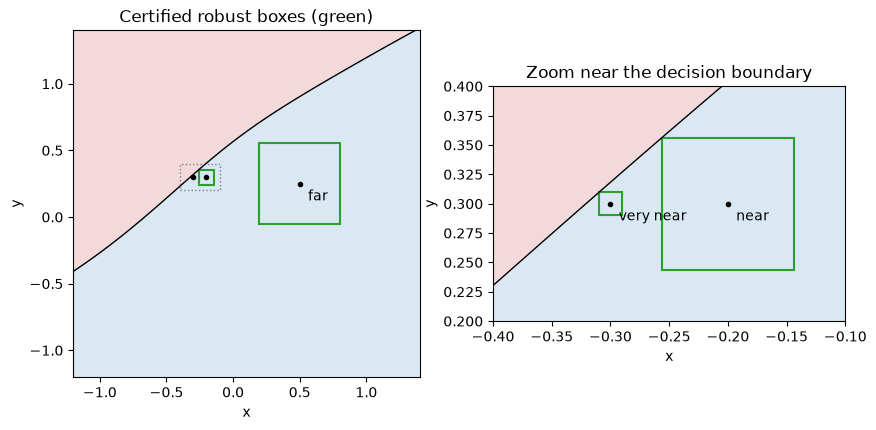
\includegraphics[width=0.9\linewidth]{figures/app08-boxes.png}
\end{center}

\begin{teaching}
Stress the logical structure: certificate $\le$ true radius $\le$ attack, and the attack's
counterexample is itself certified. Exercise 2 (the Lipschitz radius $f(c)/L$) is the method used by
many published verifiers and is a good written exercise. For a graded starter, blank out
\nb{gradient} and \nb{monotone_corners}. Students sometimes write \nb{x / 3} inside the network: with a
\nb{Dual} or \nb{RationalInterval} this may create a float and is rejected; use \nb{fmpq} or
\nb{Fraction} constants.
\end{teaching}

\app{Certified condition number}{proposal}

Lecture 03 separates conditioning from stability. Certify the relative condition number
$\kappa(x)=|x f'(x)/f(x)|$ over a whole range, for example $f(x)=1-\cos x$ on $[10^{-8},1]$, where
$\kappa(x)=x\sin x/(1-\cos x)\in[1,2]$. Then the large observed errors of the formula
\nb{1 - cos(x)} near $0$ are proved to be algorithmic, not intrinsic. The derivative comes from a dual
number; the quotient of two small quantities needs subdivision near $0$ (geometric pieces
$[2^{-k-1},2^{-k}]$). Effort: one lab; no new \nb{vc} code.

%=====================================================================
\lecture{09}{Validated roots}

\app{Ray tracing a torus: the first hit}{implemented: \nb{app09_ray_tracing_and_wilkinson}, Part A}

\field{Problem} A ray $o+td$ hits the torus
$T(x,y,z)=(x^2+y^2+z^2+R^2-r^2)^2-4R^2(x^2+y^2)$ where the quartic $g(t)=T(o+td)$ vanishes; the pixel
shows the \emph{smallest} root. Graphics codes often use ray marching: sample $g$ with step $\Delta t$ and
take the first sign change. Thin pieces of surface entered and left within one step are missed. Interval methods for ray tracing
go back to Mitchell \cite{mitchell}.

\field{Certificate} Search $t$-intervals from left to right with Lecture 09's \nb{inspect_root}. The
first certified interval contains exactly one root, and everything to its left was excluded, so it is
the first hit. Tiny undecided intervals (grazing rays) are reported as \emph{uncertain}. Two short
proofs keep the search finite and cheap: since $o+3d\perp d$, $|o+td|^2\ge(t-3)^2$, and every torus point
has norm at most $R+r<5/4$, so all hits have $t\in[7/4,17/4]$; and a ray whose distance $\sqrt{u^2+v^2}$
from the center exceeds $R+r$ is a proved miss (a bounding volume).

\field{Results} On a $40\times26$ image, marching with step $0.25$ misses 28 of the 320 certified hits,
all on the silhouette. No pixel was uncertain, and marching never reported a hit that the search
excluded.

\begin{center}
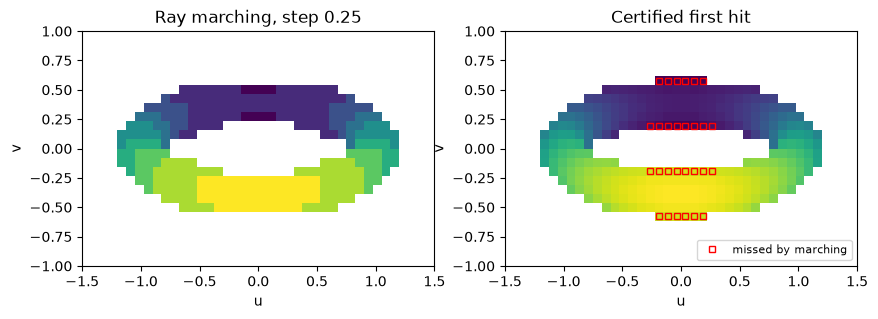
\includegraphics[width=0.95\linewidth]{figures/app09-torus.png}
\end{center}

\app{Wilkinson's polynomial: conditioning or algorithm?}{implemented: same notebook, Part B}

\field{Problem} $W(x)=\prod_{k=1}^{20}(x-k)$ has expanded coefficients up to $1.4\cdot10^{19}$, beyond
the exact-integer range of binary64. NumPy's \nb{roots} returns roots with errors up to $0.085$
(near $x=14$). Is that because storing the coefficients changed the polynomial, or because the
eigenvalue algorithm loses accuracy? Wilkinson's own account is in \cite{wilkinson}.

\field{Certificate} Interval Horner evaluation is useless here (terms of size $10^{19}$ cancel to
$10^{12}$). The notebook uses the \emph{Taylor form}: shift the polynomial exactly to the midpoint
$m$ and bound $W(m+h)=\sum c_kh^k$ by $c_0\pm\sum_{k\ge1}|c_k|\rho^k$. This is the polynomial version
of the mean-value form. A root is certified when the exact endpoint values have opposite signs and the
Taylor form of $W'$ excludes $0$. The decision is plugged into \nb{isolate_roots} through its
\nb{inspect} hook. The domain $[1/3,68/3]$ is chosen so that no bisection point is an integer.

\field{Results}
\begin{itemize}
\item Exact $W$: status \emph{complete}, 20 certified roots, 141 decisions.
\item The binary64-stored polynomial (5 coefficients change): still 20 real roots, each within
$6.2\cdot10^{-4}$ of an integer. NumPy's error is about $140$ times larger, so most of it is
algorithmic. Exact certification separates conditioning from stability.
\item Wilkinson's perturbation of the $x^{19}$ coefficient by $2^{-23}$: status \emph{complete} with
exactly ten real roots in $[1/3,68/3]$ (near $1,\dots,8$, then $8.917$ and $20.847$). The other ten
roots have become complex.
\end{itemize}

\begin{center}
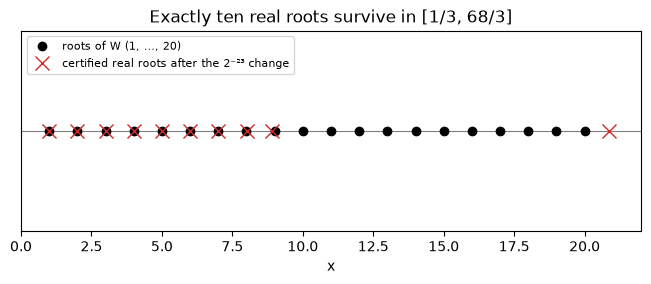
\includegraphics[width=0.85\linewidth]{figures/app09-wilkinson.png}
\end{center}

\begin{teaching}
Part A makes ``search completeness'' concrete: the left-to-right order \emph{is} the proof that the
hit is first. Ask why a smaller marching step never proves the absence of holes (a grazing ray can
make the chord arbitrarily short). Part B is the strongest link back to Lecture 03 in the course.
The claim ``exactly ten real roots'' holds only in the search domain; Exercise 4 makes it global with
Cauchy's bound. For a graded starter, blank out \nb{first_hit} and \nb{sign_change_inspector}.
\end{teaching}

\app{Kepler's equation}{proposal}

Solve $E-e\sin E=M$ for the eccentric anomaly of an orbit. Since $1-e\cos E>0$ for $e<1$, interval
Newton certifies the unique solution for each mean anomaly $M$, and with an interval $M$ for a whole
range of times at once. Near $e\to1$ and $M\to0$ the derivative enclosure approaches $0$, which shows
the certificate weakening exactly where float solvers need special starting values. Effort: half a
lab; uses \nb{evaluate_ball} and Arb's $\sin$.

%=====================================================================
\lecture{10}{Nonlinear systems}

\app{A robot arm that reaches a whole path}{implemented: \nb{app10_robot_arm_and_henon}, Part A}

\field{Problem} A two-link arm with lengths $L_1=1$, $L_2=3/4$ must reach every point of a straight
path. With the elbow position $(u,v)$ as unknowns, inverse kinematics is the polynomial system
$u^2+v^2=L_1^2$, $(u-x)^2+(v-y)^2=L_2^2$: the intersection of two circles. The workspace is the annulus
$L_1-L_2\le|(x,y)|\le L_1+L_2$, and its boundary is singular.

\field{Certificate} A \emph{parametric} Krawczyk test: the target is an interval box $T$. If the
Krawczyk image lies strictly inside the elbow box and the contraction bound is below one, then for
every target in $T$ there is exactly one elbow position in the box. A path is covered by finitely many
target boxes, so one computation certifies infinitely many targets. Pieces that fail are split; pieces
below $1/1024$ of the path are reported as not certified.

\field{Results} The path from $(-1/2,6/5)$ to $(7/4,0)$ ends exactly on the outer boundary. The search produces 47
pieces, of which 44 are certified, covering $99.7\%$ of the path. Long pieces are certified far from the boundary; the pieces shrink as the path approaches it, and the last pieces,
which touch the boundary, cannot be certified. That is the correct answer: the two solutions merge
into a double solution with singular Jacobian.

\begin{center}
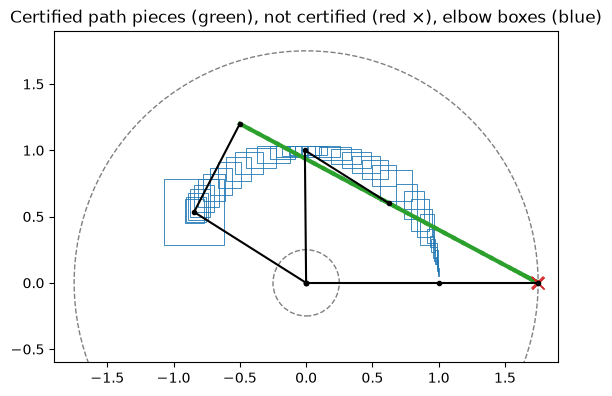
\includegraphics[width=0.62\linewidth]{figures/app10-arm.png}
\end{center}

\app{Periodic orbits of the Hénon map}{implemented: same notebook, Part B}

\field{Problem} The Hénon map $H(x,y)=(1-ax^2+y,\,bx)$ with $a=7/5$, $b=3/10$ is chaotic: float orbits
cannot be trusted point by point. Yet periodic orbits can be proved to exist.

\field{Certificate} Points with $H^k(p)=p$ solve a $2\times2$ polynomial system. Newton's method from
random starts (with the Jacobian from \nb{jacobian2} on floats) finds candidates; Krawczyk with exact
rational arithmetic certifies each one in a box of radius $10^{-8}$--$10^{-4}$.

\field{Results} All 2, 4, 8 and 16 float candidates for periods dividing 1, 2, 4 and 6 are certified.
The notebook states plainly what is not proved: random starts give no completeness, so these are
lower bounds on the number of periodic points.

\begin{center}
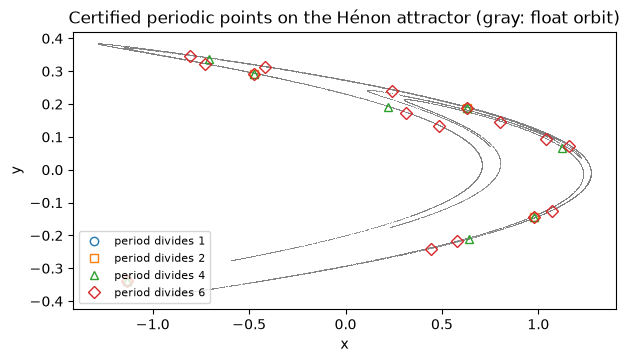
\includegraphics[width=0.8\linewidth]{figures/app10-henon.png}
\end{center}

\begin{teaching}
The parametric certificate is the conceptual highlight: it answers ``what about the points between
samples?'' for a whole family of problems. The singularity discussion connects mathematics (merging
roots) to engineering (an arm near full extension amplifies control errors). For Part B, contrast the
gray float picture (an experiment) with the markers (theorems). For a graded starter, blank out
\nb{certify_targets} and \nb{certify_path}.
\end{teaching}

\app{Trilateration}{proposal}

Locate a receiver from distances to two (or three) beacons with measurement error: the same
circle-intersection system with \emph{interval radii}. Krawczyk certifies a unique position in a box
for all radii consistent with the measurements, and fails, correctly, when the circles are nearly
tangent (bad beacon geometry, ``dilution of precision''). Effort: half a lab; reuses Part A code.

%=====================================================================
\lecture{11}{Global optimization}

\app{Fitting a frequency: local answers, global certificate}{implemented: \nb{app11_curve_fitting}}

\field{Problem} Sixteen measurements at integer times are fitted by $y\approx\sin(\omega t)$, minimizing
$S(\omega)=\sum_i(y_i-\sin\omega t_i)^2$. Gradient descent from six starts returns six ``converged''
answers; only one finds the true valley ($\omega\approx1.3003$, misfit $0.142$), the others stop at misfits
between $13.8$ and $16.1$.

\field{Certificate} \nb{minimize} from Lecture 11 with Arb enclosures of $S$, sharpened by Lecture 07's
intersection with the mean-value form. The derivative $S'$ comes from one dual-number pass through the
same \nb{misfit} code. Strict pruning keeps \emph{all} global minimizers.

\field{Results} On $\omega\in[1/10,8]$ the combined evaluator needs 95 splits (natural: 144) and keeps
\emph{two} regions, near $1.300$ and near $7.583$. The certificate has found aliasing: for integer
times $\sin((\omega+2\pi)t)=\sin(\omega t)$, so $S(\omega+2\pi)=S(\omega)$ exactly and the data cannot
distinguish the two frequencies. Restricting the model to $\omega\le3<\pi$ (a modeling decision)
leaves one region.

\begin{center}
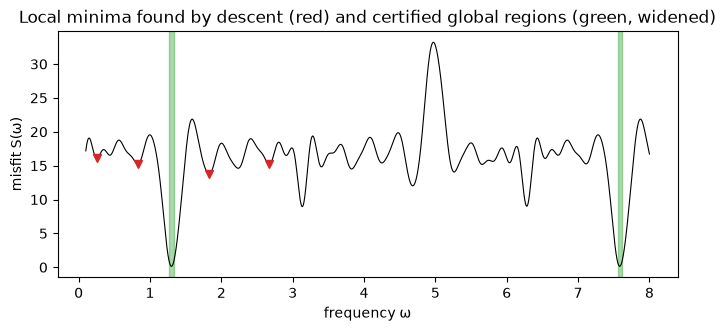
\includegraphics[width=0.9\linewidth]{figures/app11-misfit.png}
\end{center}

\begin{teaching}
This is the best example in the set for the slogan ``a certificate of the global minimum is also a
certificate of non-identifiability''. Ask students before running the search how many minimizers they
expect. Exercise 1 (interval data) shows how measurement uncertainty enlarges the set of minimizers.
For a graded starter, blank out \nb{S_combined} and the \nb{clusters} helper.
\end{teaching}

\app{SIAM 100-digit Problem 4}{proposal}

Minimize $e^{\sin 50x}+\sin(60e^y)+\sin(70\sin x)+\sin(\sin 80y)-\sin(10(x+y))+(x^2+y^2)/4$ over the
plane. The function has thousands of local minima; the global minimum is $-3.30686\ldots$. A
two-dimensional branch and bound (split boxes along their widest side, about 80 lines) with Arb
enclosures certifies several digits. The domain can be restricted by a short argument: the oscillating
terms are at least $e^{-1}-4$, and some point has value below $-3.3$, so every minimizer satisfies
$(x^2+y^2)/4\le 0.7-e^{-1}$, a disk of radius about $1.2$. This
is a sibling of the mirror capstone, which comes from the same challenge
\cite{bornemann}. Effort: a mini-project.

\app{Worst-case overshoot}{proposal}

For a damped oscillator $\ddot x+2\zeta\dot x+x=0$ with $\zeta$ in an uncertain interval, maximize the
overshoot of the closed-form step response over time and parameter. Branch and bound in $(t,\zeta)$
gives a certified worst case for a control specification. Effort: a mini-project with 2D search.

%=====================================================================
\lecture{12}{Robust geometry}

\app{A convex hull that is not convex enough}{implemented: \nb{app12_convex_hull}}

\field{Problem} Andrew's monotone-chain algorithm with a float orientation test, applied to nine ordinary
binary64 points (seven very close to the line $y=x$, plus two others), returns a triangle that leaves one
input point strictly outside. The example follows Kettner et al.\ \cite{kettner}.

\field{Certificate} Replace one function: \nb{vc.geometry.orientation} on the exact rationals that the
binary64 inputs represent. The standard correctness proof of the algorithm then applies word for word,
because it uses only signs of determinants. A separate exact checker verifies convexity and containment
independently of how the hull was computed.

\field{Results} On a $256\times256$ grid of neighboring floats near $(1/2,1/2)$, the float orientation of
$(p,(12,12),(24,24))$ is wrong for 11\,972 of 65\,536 points, and inconsistently so. The float hull fails
the checker; the exact hull (four vertices) passes. All 22 orientation calls were decided by the Arb
filter, so exactness cost almost nothing.

\begin{center}
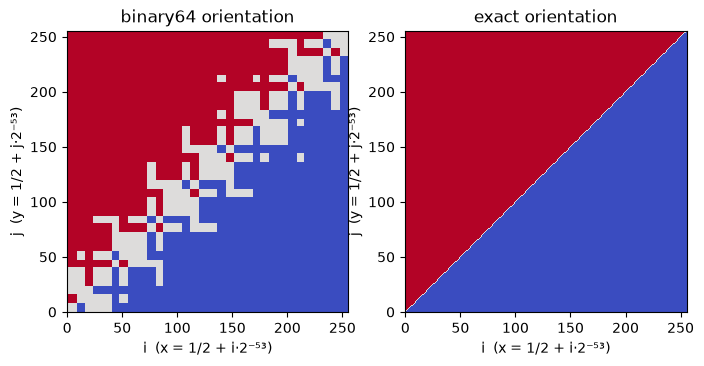
\includegraphics[width=0.8\linewidth]{figures/app12-orientation.png}

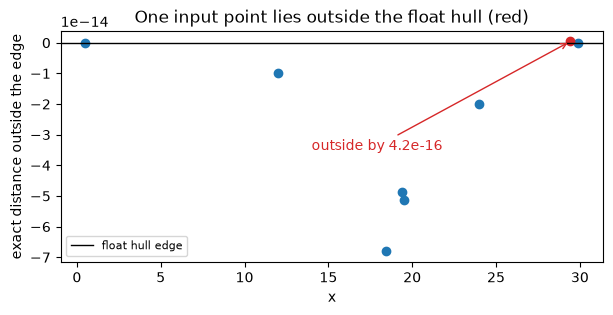
\includegraphics[width=0.7\linewidth]{figures/app12-hull.png}
\end{center}

\begin{teaching}
The orientation map is the single most memorable picture of the course for many students: show it
before explaining it. Emphasize the difference between exact inputs (the notebook) and measured
inputs (Lab 12, Task C), where some orientations are genuinely undecidable and the honest output is a
set of hulls. Exercise 1 (point in polygon) is a quick follow-up with direct GIS relevance.
\end{teaching}

\app{Segment intersection and Delaunay}{proposal}

Two further predicates show the same phenomenon: segment intersection tests (four orientations)
and the Delaunay \emph{incircle} test (a $3\times3$ determinant). A Bowyer--Watson triangulation with
float predicates on nearly cocircular points produces overlapping triangles; the filtered predicate
fixes it. Effort: a mini-project; needs an \nb{incircle} analogue of \nb{orientation} (about 30 lines).

%=====================================================================
\lecture{13}{Certificate audit}

\app{Audit four seeded certificates}{implemented: \nb{app13_seeded_audit}}

Four short ``submitted'' certificates, each printing a confident conclusion: a maximum bound by
subdivision (A), a one-root claim (B), an enclosure of $e$ (C), and an interval Newton root certificate
(D). Students audit them in pairs with a five-step checklist (claim, theorem, coverage, enclosures,
verdict) and must classify each rejection as \emph{false claim} or \emph{unsupported claim}. One
submission is correct, so that students practice accepting a valid certificate rather than inventing
flaws. The key is in \hyperref[key]{Appendix A}.

%=====================================================================
\lecture{14}{Synthesis: alternative capstones}

The mirror-trajectory capstone remains the default. The applications above can be combined into
alternative capstones of comparable size, each combining at least three lectures and each with a
natural peer-audit target.

\begin{center}
\small
\begin{tabularx}{\linewidth}{@{}l X X@{}}
\toprule
Capstone & Core certificate & Milestones\\
\midrule
Certified ray tracer & First hit (09) for several implicit surfaces; robust silhouette classification (12) & M1 one surface, uncertain pixels reported; M2 shading from certified normals (08); M3 shadows: a second first-hit query per pixel\\[3pt]
Robot workspace map & Parametric Krawczyk (10) over target boxes; subdivision (06) & M1 certified path; M2 map of the reachable region with certified/undecided cells; M3 minimal distance to singularity by branch and bound (11)\\[3pt]
Network verifier & Monotone corners (07--08) plus input splitting; global worst case (11) & M1 certified radius for test points; M2 split-and-verify for a fixed $\varepsilon$; M3 certified maximal radius by 2D branch and bound\\
\bottomrule
\end{tabularx}
\end{center}

%=====================================================================
\appendix
\phantomsection\label{key}
\section*{\color{courseblue}Appendix A\quad Instructor key for the seeded audit}
\addcontentsline{toc}{section}{Appendix A: Instructor key for the seeded audit}

\textbf{A, maximum bound by subdivision: reject, claim true but unsupported (coverage).}
The pieces are built from \nb{np.arange(0, 1, 0.1)}; the float edges are converted exactly to
fractions and then $1/10$ is added. Consecutive pieces do not meet: there are four gaps of width
$5.6\cdot10^{-18}$ to $8.9\cdot10^{-17}$ (for example after the piece starting at the float $0.2$).
Probe: check \nb{a.hi >= b.lo} for consecutive pieces. The true maximum is $0.2641$ (at
$x=(1+\sqrt7)/6$), so the claim holds, but the argument does not cover $[0,1]$. Fix: build the pieces
with exact fractions, \nb{Interval(Fraction(k, 10), Fraction(k + 1, 10))}, or use \nb{subdivide}.

\textbf{B, exactly one root: reject, claim false (enclosures: sampling used as a bound).}
Positivity of $g'$ at 20 grid points says nothing between them; the grid misses the interval
$|x|<1/\sqrt{30000}\approx0.0058$ where $g'<0$. Probe: \nb{g_B_prime(Interval(-1, 1))} contains $0$;
exact signs $g(-1)<0$, $g(-1/200)>0$, $g(1/200)<0$, $g(1)>0$ give three roots by the intermediate value
theorem (they are $0$ and $\pm1/100$). A cubic has at most three, so exactly three.

\textbf{C, enclosure of $e$: reject, claim false (enclosures: truncation remainder omitted).}
Exact summation removes rounding error but not truncation error. Probe: Arb gives
$e-s=2.7313\cdot10^{-8}$, far above the margin $10^{-12}$. Fix: add the remainder bound
$\sum_{k>10}1/k!<\frac{1}{11!}\cdot\frac{12}{11}$.

\textbf{D, root of $x^2-2$: accept.} The derivative enclosure $[2,4]$ is valid on $[1,2]$, the
Newton image $[1.375,1.4375]$ lies strictly inside $[1,2]$, so there is exactly one root in $[1,2]$, and
it lies in the intersection. Students who reject D should be asked for a probe; there is none.

\section*{\color{courseblue}Appendix B\quad Files and building}
\addcontentsline{toc}{section}{Appendix B: Files and building}

The notebook sources are the Jupytext files \nb{applications/app*.py}; the \nb{.ipynb} files are
generated from them and contain executed outputs. From the course root:
\begin{itemize}
\item \nb{.venv/bin/python applications/build.py} syncs, executes all notebooks, extracts the figures
tagged \nb{tex-figure-*}, and compiles this document to \nb{applications/applications.pdf};
\item \nb{build.py sync}, \nb{build.py execute app09}, and \nb{build.py pdf} run single steps.
\end{itemize}
The build puts the repository root on \nb{PYTHONPATH}, so \nb{vc} is importable without an
installation. The notebooks are not yet part of \nb{scripts/notebooks.py} or the release packages.

\begin{thebibliography}{9}\small
\bibitem{bornemann} F.~Bornemann, D.~Laurie, S.~Wagon, J.~Waldvogel, \emph{The SIAM 100-Digit
Challenge: A Study in High-Accuracy Numerical Computing}, SIAM, 2004.
\bibitem{chevillard} S.~Chevillard, J.~Harrison, M.~Joldeş, Ch.~Lauter, Efficient and accurate
computation of upper bounds of approximation errors, \emph{Theoretical Computer Science} 412 (2011).
\bibitem{goodfellow} I.~Goodfellow, J.~Shlens, C.~Szegedy, Explaining and harnessing adversarial
examples, ICLR 2015.
\bibitem{gowal} S.~Gowal et al., On the effectiveness of interval bound propagation for training
verifiably robust models, arXiv:1810.12715, 2018.
\bibitem{kettner} L.~Kettner, K.~Mehlhorn, S.~Pion, S.~Schirra, C.~Yap, Classroom examples of
robustness problems in geometric computations, \emph{Computational Geometry} 40 (2008) 61--78.
\bibitem{mitchell} D.~P.~Mitchell, Robust ray intersection with interval arithmetic,
\emph{Graphics Interface} 1990.
\bibitem{tucker} W.~Tucker, \emph{Validated Numerics: A Short Introduction to Rigorous
Computations}, Princeton University Press, 2011.
\bibitem{wilkinson} J.~H.~Wilkinson, The perfidious polynomial, in \emph{Studies in Numerical
Analysis}, MAA, 1984.
\end{thebibliography}

\end{document}
